\documentclass[problem]{mcs}

\begin{pcomments}
  \pcomment{MQ_expectHH_TT_S16}
  \pcomment{similar to MQ_expectHHH/_F15}
  \pcomment{ARM 12/15/15}
\end{pcomments}

\pkeywords{
  expectation
  conditional_expectation
  total_expectation
  probability_tree
  tree_model
}

%%%%%%%%%%%%%%%%%%%%%%%%%%%%%%%%%%%%%%%%%%%%%%%%%%%%%%%%%%%%%%%%%%%%%
% Problem starts here
%%%%%%%%%%%%%%%%%%%%%%%%%%%%%%%%%%%%%%%%%%%%%%%%%%%%%%%%%%%%%%%%%%%%%

\begin{problem}
A coin with probability $p$ of flipping Heads and probability $q
\eqdef 1-p$ of flipping tails is repeatedly flipped until two
consecutive flips match---that is, until HH or TT occurs.  The outcome
tree, $A$, for this setup is illustrated in Figure~\ref{HH-TT-tree}.

    \begin{figure}
      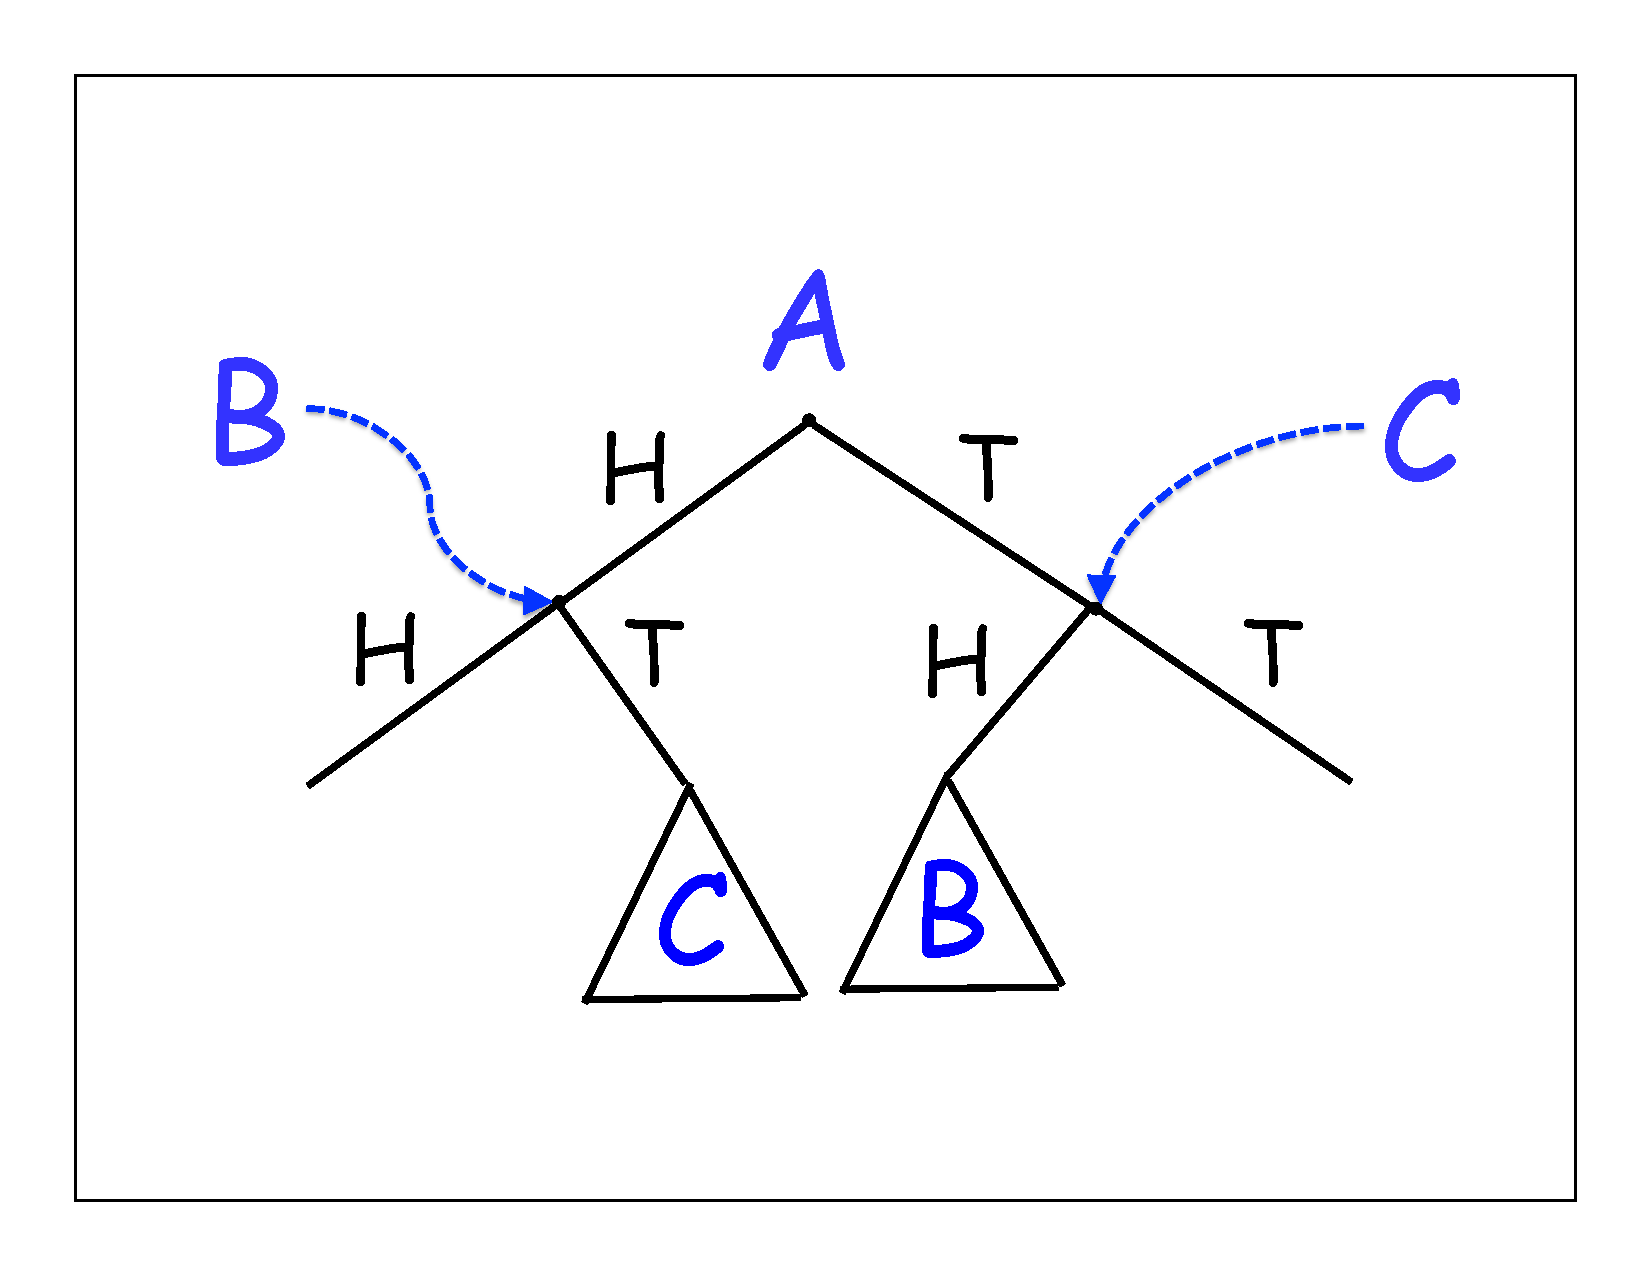
\includegraphics[width=3.5in]{HH-TT-tree-frame}
     \caption{Outcome Tree for Flipping Until HH or TT}
     \label{HH-TT-tree}
    \end{figure}

Let $e(X)$ be the expected number of flips starting at the root of
subtree $X$, where $X$ is $A$, $B$, or $C$.

\iffalse
\hint Write a small system of equations involving $e(A), e(B)$, and
$e(C)$ based on Total Expectation and solve for $e(A)$.
\fi

%\bparts \ppart

Express each of $e(A),e(B),e(C)$ as a linear combination of the other
two. (For example, express $e(B)$ in terms of $e(A)$ and/or $e(C)$).
You need not solve the system of equations.

\begin{solution}
By the Total Expectation Rule, we have
\begin{align*}
e(A) & = p(1+ e(B)) + q(1+e(C)) = 1 + p\cdot e(B) + q\cdot e(C),\\
e(B) & = p(1+0) + q(1+ e(C))    = 1 + q\cdot e(C),\\
e(C) & = p(1+e(B)) + q(1+ 0)    = 1 + p\cdot e(B).
\end{align*}
\end{solution}

\iffalse
\examspace[1.5in]

\ppart Express the value of $e(A)$ with a simple formula involving $p$
and $q$.

\begin{solution}
Substituting for $e(C)$, we get
\[
e(B) = 1 + q + (pq)\, e(B),
\]
so
\[
e(B) = \frac{1+q}{1-pq}\ .
\]
Similarly,
\[
e(C) = \frac{1+p}{1-pq}\ .
\]
Therefore,
\begin{align*}
e(A) & = 1 + \frac{p(1+q)}{1-pq} + \frac{q(1+p)}{1-pq}\\
     & = \frac{1-pq+p(1+q)+ q(1+p)}{1-pq}\\
     & = \frac{1-pq+p+pq+q+pq}{1-pq}\\
     & = \frac{2+pq}{1-pq}.
\end{align*}

It's worth noting---though the question did not call for this---that
$e(A)$ is smallest when $pq$ is smallest.  That happens when $p=0$ or
$q=0$, in which case $e(A) = 2$.  On the other hand, $e(A)$ is largest
when $pq$ is largest.  That happens when $p=q=1/2$, in which case
$e(A) = 3$.
\end{solution}

\eparts
\fi

\end{problem}

%%%%%%%%%%%%%%%%%%%%%%%%%%%%%%%%%%%%%%%%%%%%%%%%%%%%%%%%%%%%%%%%%%%%%
% Problem ends here
%%%%%%%%%%%%%%%%%%%%%%%%%%%%%%%%%%%%%%%%%%%%%%%%%%%%%%%%%%%%%%%%%%%%%

\endinput

